\documentclass[12pt, a4paper, oneside]{memoir}
\usepackage[T1]{fontenc}
\usepackage[utf8]{inputenc}
\usepackage{newtxtext,newtxmath}
\usepackage{xurl} 
\usepackage{microtype}
\usepackage{csquotes}

\setSpacing{1.5}
\settocdepth{subsection}
\setsecnumdepth{subsection}
\renewcommand{\contentsname}{Table of Contents}

\setstocksize{297mm}{210mm}
\settrimmedsize{297mm}{210mm}{*}

\setlrmarginsandblock{1.5in}{1in}{*}
\setulmarginsandblock{1in}{1in}{*}

\setheadfoot{15pt}{0.5in}
\setheaderspaces{*}{0pt}{*}

\checkandfixthelayout

\usepackage{graphicx}
\graphicspath{{images/}}
\usepackage{booktabs}
\usepackage{array}
\usepackage{caption}
\usepackage{subcaption}
\usepackage{xcolor}
\usepackage{colortbl}
\usepackage{arydshln}
\usepackage[linesnumbered,ruled,vlined]{algorithm2e}
\usepackage{float}
\usepackage{forloop}
\newcounter{loopcntr}
\newcommand{\on}[1]{%
  \forloop{loopcntr}{0}{\value{loopcntr}<#1}{& \cellcolor{gray}}%
}
\newcommand{\off}[1]{%
  \forloop{loopcntr}{0}{\value{loopcntr}<#1}{&}%
}
\usepackage{tikz}
\usetikzlibrary{tikzmark, shapes.geometric, arrows.meta, positioning, fit, backgrounds}

\usepackage{enumitem}
\setlist{nosep}
\nonzeroparskip
\setlength{\parindent}{0pt}
\setlength{\parskip}{12pt}

\usepackage{hyperref}
\hypersetup{
    colorlinks=true,
    linkcolor=darkblue,
    citecolor=darkblue,
    urlcolor=black,
    pdfborder={0 0 0},
    pdftitle={TRIBAL: Roommate Matching and Event Discovery Platform},
    pdfauthor={Gahan},
    pdfkeywords={Flutter, Django, PostgreSQL, Roommate Matching, Compatibility Scoring, JWT, WebSockets}
}
\usepackage{bookmark}

\definecolor{darkblue}{rgb}{0,0,0.5}

\makepagestyle{proposalstyle}
\makeoddhead{proposalstyle}{}{}{}
\makeevenhead{proposalstyle}{}{}{}
\makeheadrule{proposalstyle}{\textwidth}{0pt}
\makeoddfoot{proposalstyle}{}{\thepage}{}
\makeevenfoot{proposalstyle}{}{\thepage}{}
\pagestyle{proposalstyle}
\aliaspagestyle{chapter}{proposalstyle}

\chapterstyle{veelo}

\makechapterstyle{custom16pt}{
  \setlength{\beforechapskip}{-20pt}
  \setlength{\afterchapskip}{12pt}
  \renewcommand*{\printchaptername}{}
  \renewcommand*{\chapternamenum}{}
  \renewcommand*{\printchapternum}{\normalfont\fontsize{16}{20}\bfseries Chapter \thechapter\quad}
  \renewcommand*{\afterchapternum}{}
  \renewcommand*{\printchaptertitle}[1]{\normalfont\fontsize{16}{20}\bfseries ##1}
}
\chapterstyle{custom16pt}

\setsecheadstyle{\normalfont\fontsize{14}{17}\bfseries}
\setsubsecheadstyle{\normalfont\fontsize{13}{16}\bfseries}
\setsubsubsecheadstyle{\normalfont\fontsize{12}{15}\bfseries}

\usepackage[
    backend=biber,
    style=ieee,
    sorting=none
]{biblatex}
\DeclareFieldFormat{url}{#1}
\addbibresource{references.bib}
\addbibresource{bibliography.bib}

\begin{document}

\frontmatter

\thispagestyle{empty}
\begin{center}
    \begin{Spacing}{1.1}
        {\large\bfseries TRIBHUWAN UNIVERSITY\par}
        {\large\bfseries INSTITUTE OF ENGINEERING\par}
        {\large\bfseries KATHMANDU ENGINEERING COLLEGE\par}
        {\small KALIMATI, KATHMANDU\par}
    \end{Spacing}

    \vspace{0.4cm}
    
\includegraphics[width=2.5cm]{kec_logo.png}

    \vspace{0.4cm}
    {\normalsize Minor Project Proposal Report\par}
    \vspace{0.1cm}
    {\normalsize On\par}

    \vspace{0.4cm}
    \begin{Spacing}{1.2}
        {\large\bfseries Tribal: Find Your Tribe\par}
    \end{Spacing}

    \vspace{0.2cm}
    {\normalsize [Code Number: ENCT354]\par}

    \vspace{0.4cm}
    {\normalsize BY\par}
    \vspace{0.2cm}
    \begin{tabular}{l@{\hspace{1.5cm}}l}
        Sampada Dahal & [KAT080BCT067] \\
        Selina Pageni & [KAT080BCT073] \\
        Shlesha Aryal & [KAT080BCT075] \\
        Sukriti Dhakal & [KAT080BCT083] \\
    \end{tabular}

    \vfill

    {\normalsize TO\par}
    \vspace{0.2cm}
    {\large\bfseries DEPARTMENT OF COMPUTER ENGINEERING\par}
    \vspace{0.1cm}
    {\normalsize KATHMANDU, NEPAL\par}
    \vspace{0.1cm}
    {\normalsize June 2026\par}
\end{center}
\clearpage

% \thispagestyle{empty}
\begin{center}
    \vspace*{0pt}
    
\includegraphics[width=2.8cm]{kec_logo.png}

    \vspace{0.6cm}
    \begin{Spacing}{1.1}
    {\huge\bfseries Tribal: Find Your Tribe\par}
    \end{Spacing}

    \vspace{0.6cm}
    {\large\scshape A Minor Project Mid Defense Report\par}

    \vspace{0.8cm}
    {\small Submitted in partial fulfillment of the requirements for the degree of\par}
    {\small\textbf{Bachelor in Computer Engineering}\par}

    \vspace{1cm}
    {\small Proposed by:\par}
    {\small\bfseries 
        Sampada Dahal (BCT80067)\par 
        Selina Pageni (BCT80073)\par 
        Shlesha Aryal (BCT80075)\par
        Sukriti Dhakal (BCT80083)\par
    }

    \vfill

    \begin{Spacing}{0.9}
        {\normalsize Department of Computer Engineering\par}
        {\normalsize\bfseries Kathmandu Engineering College\par}
        {\small (Affiliated to Tribhuvan University)\par}
        {\small Kalimati, Kathmandu, Nepal\par}
    \end{Spacing}

    \vspace{0.2cm}
    {\normalsize June 2026\par}
\end{center}
\clearpage

\chapter*{Acknowledgement}
\addcontentsline{toc}{chapter}{Acknowledgement}

 We would like to express our sincere gratitude to our project supervisor for providing us with continuous guidance and support throughout the development of this project. Without the supervisor's valuable suggestions and feedback, it would have been difficult for us to bring this project to its current state.

We are also thankful to the Department of Computer Engineering and all the faculty members who have supported us during this minor project. Their encouragement has helped us stay focused and motivated.

We would like to thank the Minor Project Coordinator, Krista Byanju, for organizing the mid-term defense and keeping us informed about the requirements and deadlines.

We also want to thank our friends and classmates who gave us feedback on the design and features of the application during its early stages. Their opinions helped us improve the overall idea of the project.

Finally, we are grateful to our families for their constant support and encouragement throughout this academic journey.


% \vspace{1.5cm}
% \noindent
% \begin{minipage}[t]{0.45\textwidth}
% \rule{5cm}{0.4pt}\\
% \textbf{Aayush Lohani}\\
% (BCT80004)
% \end{minipage}
% \hfill
% \begin{minipage}[t]{0.45\textwidth}
% \rule{5cm}{0.4pt}\\
% \textbf{Bimarsha Dahal}\\
% (BCT80026)
% \end{minipage}

% \vspace{1.5cm}
% \noindent
% \begin{minipage}[t]{0.45\textwidth}
% \rule{5cm}{0.4pt}\\
% \textbf{Gahan Raj Dangol}\\
% (BCT80033)
% \end{minipage}
% \hfill
% \begin{minipage}[t]{0.45\textwidth}
% \rule{5cm}{0.4pt}\\
% \textbf{Manish Poudel}\\
% (BCT80044)
% \end{minipage}
\clearpage

\chapter*{Abstract}
\addcontentsline{toc}{chapter}{Abstract}
Finding compatible roommates and meeting like-minded people in a new city is a problem that many people face today. Most of the existing platforms either focus only on roommate searching or only on social activities. There is no single platform that can help users find roommates, join activities, and build a trusted community all at once.

TRIBAL is a mobile application built using Flutter that tries to solve this problem. The application allows users to find compatible roommates based on their lifestyle preferences, find activity partners, create and join local events, and chat with other users. The platform also includes a compatibility scoring algorithm that matches users based on factors like budget, sleep schedule, cleanliness habits, pet preferences, and other lifestyle-related questions collected during onboarding.

The backend of the application is built using Django and uses PostgreSQL as the database. Authentication is handled using JWT tokens and real-time chat is being implemented using Django Channels with WebSockets.

At the time of this mid-term report, the team has completed the UI design, authentication flow, onboarding screens, backend setup, database models, and API integration. Work is still ongoing on the compatibility engine, chat system, and event module.

This report presents the background, methodology, current progress, and remaining work for the TRIBAL project.


\vspace{1em}

\clearpage

\clearpage
\tableofcontents
\clearpage
\listoffigures
\clearpage
\listoftables
\clearpage

\chapter*{Abbreviations}
\addcontentsline{toc}{chapter}{Abbreviations}

\begin{description}[leftmargin=3.5cm, style=nextline, font=\normalfont]
    \item[API]      Application Programming Interface
    \item[Dart]     Dart Programming Language
    \item[Django]   Django Web Framework
    \item[Figma]    Figma Design Tool
    \item[Flutter]  Flutter UI Framework
    \item[Git]      Git Version Control System
    \item[GitHub]   GitHub Code Hosting Platform
    \item[JWT]      JSON Web Token
    \item[MVC]      Model-View-Controller
    \item[PostgreSQL] PostgreSQL Database
    \item[Postman]  Postman API Testing Tool
    \item[Python]   Python Programming Language
    \item[REST]     Representational State Transfer
    \item[UI]       User Interface
    \item[UML]      Unified Modeling Language
    \item[UX]       User Experience
    \item[VS Code]  Visual Studio Code
\end{description}
\clearpage


\mainmatter

 \chapter{Introduction}
 
 \section{Background Theory}
 
In recent years, the increasing number of students and working professionals moving to new cities has created a growing need for platforms that help users find compatible roommates and build social connections. Existing social media and roommate-finding applications either lack compatibility-based matching or focus only on basic profiles, leaving a gap in the market.

TRIBAL is a cross-platform mobile application developed using Flutter and Django to address this problem. It enables users to create profiles, answer lifestyle-based onboarding questions, and find compatible roommates and activity partners through a weighted compatibility scoring algorithm. The application also supports event creation, participation, and real-time chat between matched users.

The weighted compatibility scoring approach was chosen over machine learning because it is transparent, easier to implement within the scope of a minor project, and provides meaningful matches based on users' preferences and interests.

 \section{Problem Statements}
People who want to find others with shared interests often have no proper platform to do so. General social media platforms are too broad and not designed for this kind of need. Activity-specific platforms like Meetup are not widely used in Nepal and do not support roommate finding at all.

The main problems that TRIBAL tries to address are:
\begin{itemize}
\item Finding compatible roommates and building a social circle is challenging for students and young professionals who move to new cities, as they often rely on informal methods such as friends or social media groups.


\item Existing platforms do not provide a single solution for roommate matching, activity partner discovery, and community building, while also overlooking important lifestyle compatibility factors.

\item TRIBAL addresses these challenges by offering a unified platform with compatibility-based roommate matching, activity partner discovery, event participation, and secure in-app chat.


\end{itemize}


TRIBAL aims to solve these problems by providing a single mobile platform where users can find compatible roommates, discover activity partners, join events, and chat with matches in a safe environment.

 \section{Objectives}
 The main objectives of this project are:
\begin{itemize}
  \item To design and develop a Flutter-based mobile application with a Django and PostgreSQL backend that enables users to find compatible roommates and activity partners through secure authentication, profile management, and a weighted compatibility matching algorithm.
  \item To implement core social features, including real-time chat, event creation and participation, and interest-based activity discovery, while ensuring secure communication and data management.
\end{itemize}

 \section{Scope and Applications}
 
The scope of this project as a minor project includes the following features:
\begin{itemize}


\item Develop a cross-platform Flutter application that enables users to find compatible roommates and activity partners through secure authentication, profile management, and preference-based matching.
\item Provide essential social features, including real-time chat, event creation and participation, and interest-based activity discovery to help users build meaningful connections.
\item Address the challenges of finding roommates and social networks, particularly for students and newcomers in Nepal, while serving as a scalable prototype for future enhancements such as verified profiles and location-based recommendations.

\end{itemize}

For the purpose of this minor project, the focus is on completing the core features
including the compatibility matching system, real-time chat, and event module. The
application is not intended for commercial deployment at this stage, but it demonstrates a
working prototype of the complete system.
 
 \chapter{Literature Review}
Before starting the design of TRIBAL, the team looked at some existing applications that
solve similar problems. This helped the team understand what features are already
available, what is missing, and how TRIBAL can be different from these platforms. This
chapter looks at a few popular apps that are related to roommate finding and activity
matching, and explains their limitations.

\section{Roomster}
Roomster is a roommate and room-finding platform that is mainly used in the United
States and a few other countries. It allows users to post listings for rooms and search for
roommates based on location and budget. However, Roomster does not have any real
compatibility matching system. It mostly works like a classified listing site where users
browse profiles and contact each other manually. There is no scoring system to tell a user
how well they might get along with a potential roommate based on lifestyle habits like
cleanliness, sleep schedule, or smoking


\section{Bumble BFF}
Bumble BFF is a friend-finding mode of the popular Bumble dating app. It uses a swipebased system where users can like or pass on other profiles to find friends with similar
interests. While this works well for general friend matching, it is not designed for
roommate finding. Bumble BFF also does not collect detailed lifestyle information like
budget range or sleep schedule, which are important factors when two people are going to
live together.

\section{Meetup}
Meetup is a platform mainly used to organize and join group activities and events based
on shared interests. It works well for finding activity partners but does not have any
roommate matching feature at all. Meetup is also not very popular in Nepal, and most
local activity groups still rely on Facebook groups or word of mouth instead.

\section{Facebook Groups}
Facebook Groups are widely used in Nepal for both roommate searching and activity
planning. Many people post in groups like “Room for Rent Kathmandu” or “Hiking
Buddies Nepal” to find roommates or activity partners. The biggest problem with this
method is that there is no structured system behind it. Anyone can post anything, there is
no compatibility check, and there is no way to verify whether the listed information is
true. This often leads to mismatched roommates and unsafe meetups with strangers.

\section{Roomi}
Roomi is another roommate-finding application that allows users to filter listings by
location, price, and a few basic preferences. It is more focused on the United States
market and is not commonly used in Nepal. Like Roomster, Roomi does not use any
weighted scoring system, so users still have to manually go through profiles and decide
compatibility on their own.

\section{SpareRoom}
SpareRoom is a roommate listing platform used mostly in the United Kingdom. It allows
detailed filtering of listings, such as gender preference and smoking status, but the
matching is still based on simple filters rather than an actual compatibility score. There is
no algorithm that combines multiple lifestyle factors into a single match percentage.

\section{Summary of Limitations}
After looking at these platforms, the team noticed a few common limitations:
\begin{itemize}
\item Most platforms either focus only on roommate listing or only on activity and
event matching, but not both.
\item None of these apps use a proper compatibility scoring system that takes multiple
lifestyle factors into account at once.
\item Apps that are popular internationally, like Roomster, Roomi, and SpareRoom, are
not commonly used or trusted in Nepal.
\item Local methods like Facebook groups do not provide any safety or compatibility
checks, which can lead to bad roommate experiences.
\item There is no platform that allows users to both find a compatible roommate and
discover local activity partners from one single application.
\end{itemize}
\section{How Tribal is different}
TRIBAL tries to solve these problems by combining roommate matching and activity and
event discovery into a single mobile application. Instead of relying on manual browsing,
TRIBAL uses a weighted compatibility scoring algorithm that compares onboarding
answers from two users and generates a compatibility score out of 100. This score
considers multiple lifestyle factors together, such as cleanliness, budget, sleep schedule,
noise level, smoking, guests, interests, study habit, food, and drinking preference, instead
of just one or two filters.
By keeping the matching system rule-based instead of using machine learning, TRIBAL
is able to give users a transparent and explainable match score. A user can see why their
compatibility score with another person is high or low, which is something most existing
platforms do not provide. This approach is also more practical to build and test within the
time frame of a minor project, while still giving meaningful results to users.
 
 
\chapter{Methodology}

\section{Process Model}
The team is following the Agile process model for the development of TRIBAL. Agile
was chosen because it allows the project to be broken down into small, manageable parts
called sprints, and each sprint produces a working piece of the application. This is useful
for a minor project because requirements can be refined as the team learns more, and
progress can be shown at regular intervals like this mid-term defense.
The project has been divided into the following sprints:
\begin{itemize}
\item Sprint 1: Project setup, requirement analysis, and UI/UX wireframing in Figma.
\item Sprint 2: Flutter onboarding flow, authentication screens (Login and Signup), and
post-signup profile completion screens.
\item Sprint 3: Django backend setup, PostgreSQL database design, and JWT-based
authentication APIs.
\item Sprint 4: Design and implementation of the roommate compatibility scoring
algorithm (current sprint).
\item Sprint 5: Real-time chat system using Django Channels and WebSockets.
\item Sprint 6: Event creation and joining module.
\item Sprint 7: Integration testing between the Flutter frontend and Django backend.
\item Sprint 8: Final testing, bug fixing, and documentation.
\end{itemize}
At the time of this report, the team has completed Sprints 1 to 4 and has started work on
Sprint 5.

\begin{figure}[H]
    \centering
    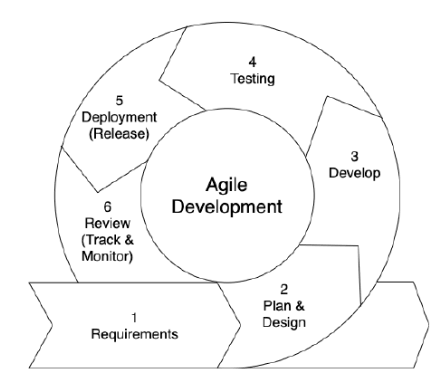
\includegraphics[width=0.8\textwidth]{images/process.png}
    \caption{Agile Process Model}
    \label{fig:agile_process}
\end{figure}


\section{System Block Diagram}

\begin{figure}[H]
    \centering
    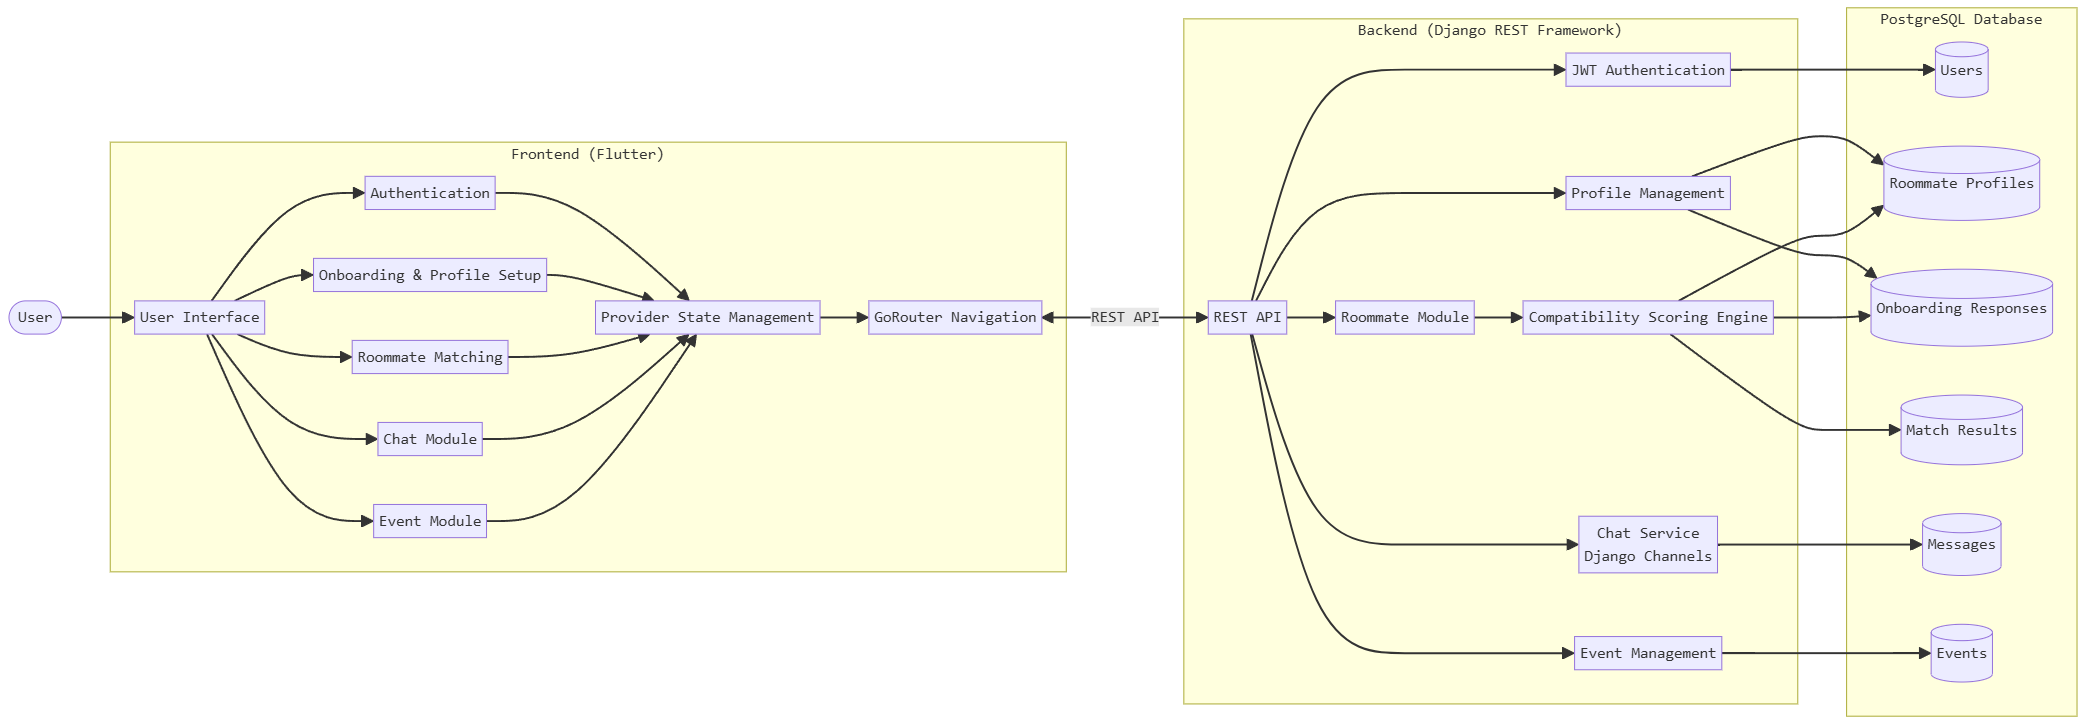
\includegraphics[width=0.8\textwidth]{images/system.png}
    \caption{System Block Diagram}
    \label{fig:block_diagram}
\end{figure}
The system is divided into three main layers:
\begin{itemize}
\item Frontend (Flutter): Handles the user interface, including onboarding,
authentication screens, and profile setup. The frontend uses Provider for state
management, GoRouter for navigation, and follows an MVC-based architecture.
\item Backend (Django): Exposes REST APIs for authentication, user profiles, and
roommate matching. The roommate matching logic lives entirely inside a single
roommate module, which keeps the matching-related code organized and separate
from the rest of the backend.
\item Database (PostgreSQL): Stores user accounts, roommate profile data, and
onboarding responses that are later used by the scoring algorithm.
\end{itemize}
The Flutter app communicates with the Django backend through REST APIs. JWT
tokens are used to keep the user logged in and to secure each API request. When a user
requests roommate matches, the request goes to the roommate module, which fetches
relevant profiles from the database, runs the scoring algorithm, and returns a ranked list
of compatible roommates back to the app.


\section{Algorithm}

\subsection{Roommate Compatibility Scoring Algorithm}
The core feature of TRIBAL at this stage is the roommate compatibility scoring
algorithm. The team decided not to use machine learning for this feature. Instead, a rule-based weighted scoring system was designed. This decision was made because a rule-based system is easier to explain, easier to test, and does not need a large dataset to train
on, which makes it more suitable for a minor project than a machine learning model.
The algorithm compares two users’ onboarding answers and produces a single
compatibility score between 0 and 100. The onboarding answers used in scoring include
cleanliness, budget, sleep schedule, noise level, smoking, guests, interests, study habit,
food preference, and drinking habit. The pet preference field is collected during
onboarding and stored in the profile, but it is not currently used in the scoring calculation.
Each factor is given a weight depending on how much it usually affects roommate
compatibility in real life. For ex le, cleanliness and budget are given higher weights
because mismatches in these areas are more likely to cause conflict, while smaller
lifestyle preferences are given lower weights.

Table 3.1 below shows the weight distribution used in the scoring algorithm.
\begin{table}[H]
\centering
\begin{tabular}{|l|c|}
\hline
\textbf{Factor} &  \textbf{Weight (\%)} \\
\hline
Cleanliness & 15 \\
Budget & 15 \\
Sleep Schedule & 12 \\
Noise Level & 10 \\
Smoking & 10 \\
Guests & 8 \\
Interests & 10 \\
Study Habit & 8 \\
Food Preference & 7 \\
Drinking & 5 \\
\hline
\end{tabular}
\caption{Compatibility Scoring Weights}
\label{table:scoring_weights}
\end{table}
The general formula used to calculate the final compatibility score is:

\begin{equation}
\text{Final Score} = \sum \left(\text{Factor Match Value} \times \text{Factor Weight}\right)
\end{equation}

Where Factor Match Value is a number between 0 and 1 that represents how closely two
users’ answers match for a particular factor, and Factor Weight is the percentage weight
assigned to that factor as shown in Table 3.1.
For factors with a small number of fixed options, such as smoking or sleep schedule, the
match value is calculated using a simple rule: if both users selected the same option, the
match value is 1; if their answers are close but not the same (for ex le, “early riser”
and “no preference”), a partial match value such as 0.5 is given; and if the answers
directly conflict (for ex le, “smoker” matched with “non-smoker, no smoking
allowed”), the match value is set to 0.
For factors that involve multiple selections, such as interests, the match value is
calculated as the number of common interests divided by the total number of unique
interests selected by both users combined. This gives a percentage overlap between the
two users’ interests.
For numeric factors like budget, the match value decreases as the difference between the
two users’ stated budgets increases. If the difference is within an acceptable range, the
match value stays close to 1. If the difference is very large, the match value moves closer
to 0.


\subsection{Deal Breakers}
Apart from the weighted scoring, the algorithm also includes a deal breaker check. Some lifestyle differences are considered serious enough that they should not simply lower the score a little, but should instead strongly affect or override the final match. For ex le, if one user is a heavy smoker and the other has explicitly said they cannot live with a smoker at all, this is treated as a deal breaker rather than just a normal mismatch. Table 3.2 lists the deal breaker rules currently used in the algorithm.
\begin{table}[H]
\centering
\begin{tabular}{|l|l|}
\hline
\textbf{Condition}  & \textbf{Effect on Score} \\
\hline
Smoking conflict (smoker vs. strictly non-smoking) & Score capped at a low maximum \\
Extreme budget mismatch (outside acceptable range) & Score capped at a low maximum \\
Opposite cleanliness extremes (very messy vs. very strict) & Score significantly reduced \\
\hline
\end{tabular}
\caption{Deal Breaker Rules}
\label{table:deal_breakers}
\end{table}
When a deal breaker condition is detected, the algorithm does not let the final score go above a fixed low ceiling, even if all other factors match well. This makes sure that users are not shown as highly compatible with someone they have a fundamental lifestyle conflict with.


\subsection{Final Score Calculation}
Once all the individual factor match values are calculated and weighted, they are added together to get the final compatibility score. If a deal breaker is triggered, the score is capped according to the deal breaker rule before being returned to the user. The final score is then rounded to the nearest whole number and shown to the user as a percentage match out of 100. This score is what the user sees in the app when browsing potential roommates, helping them quickly understand how compatible they may be with someone before starting a conversation.


\section{Flowchart}
\begin{figure}[H]
    \centering
    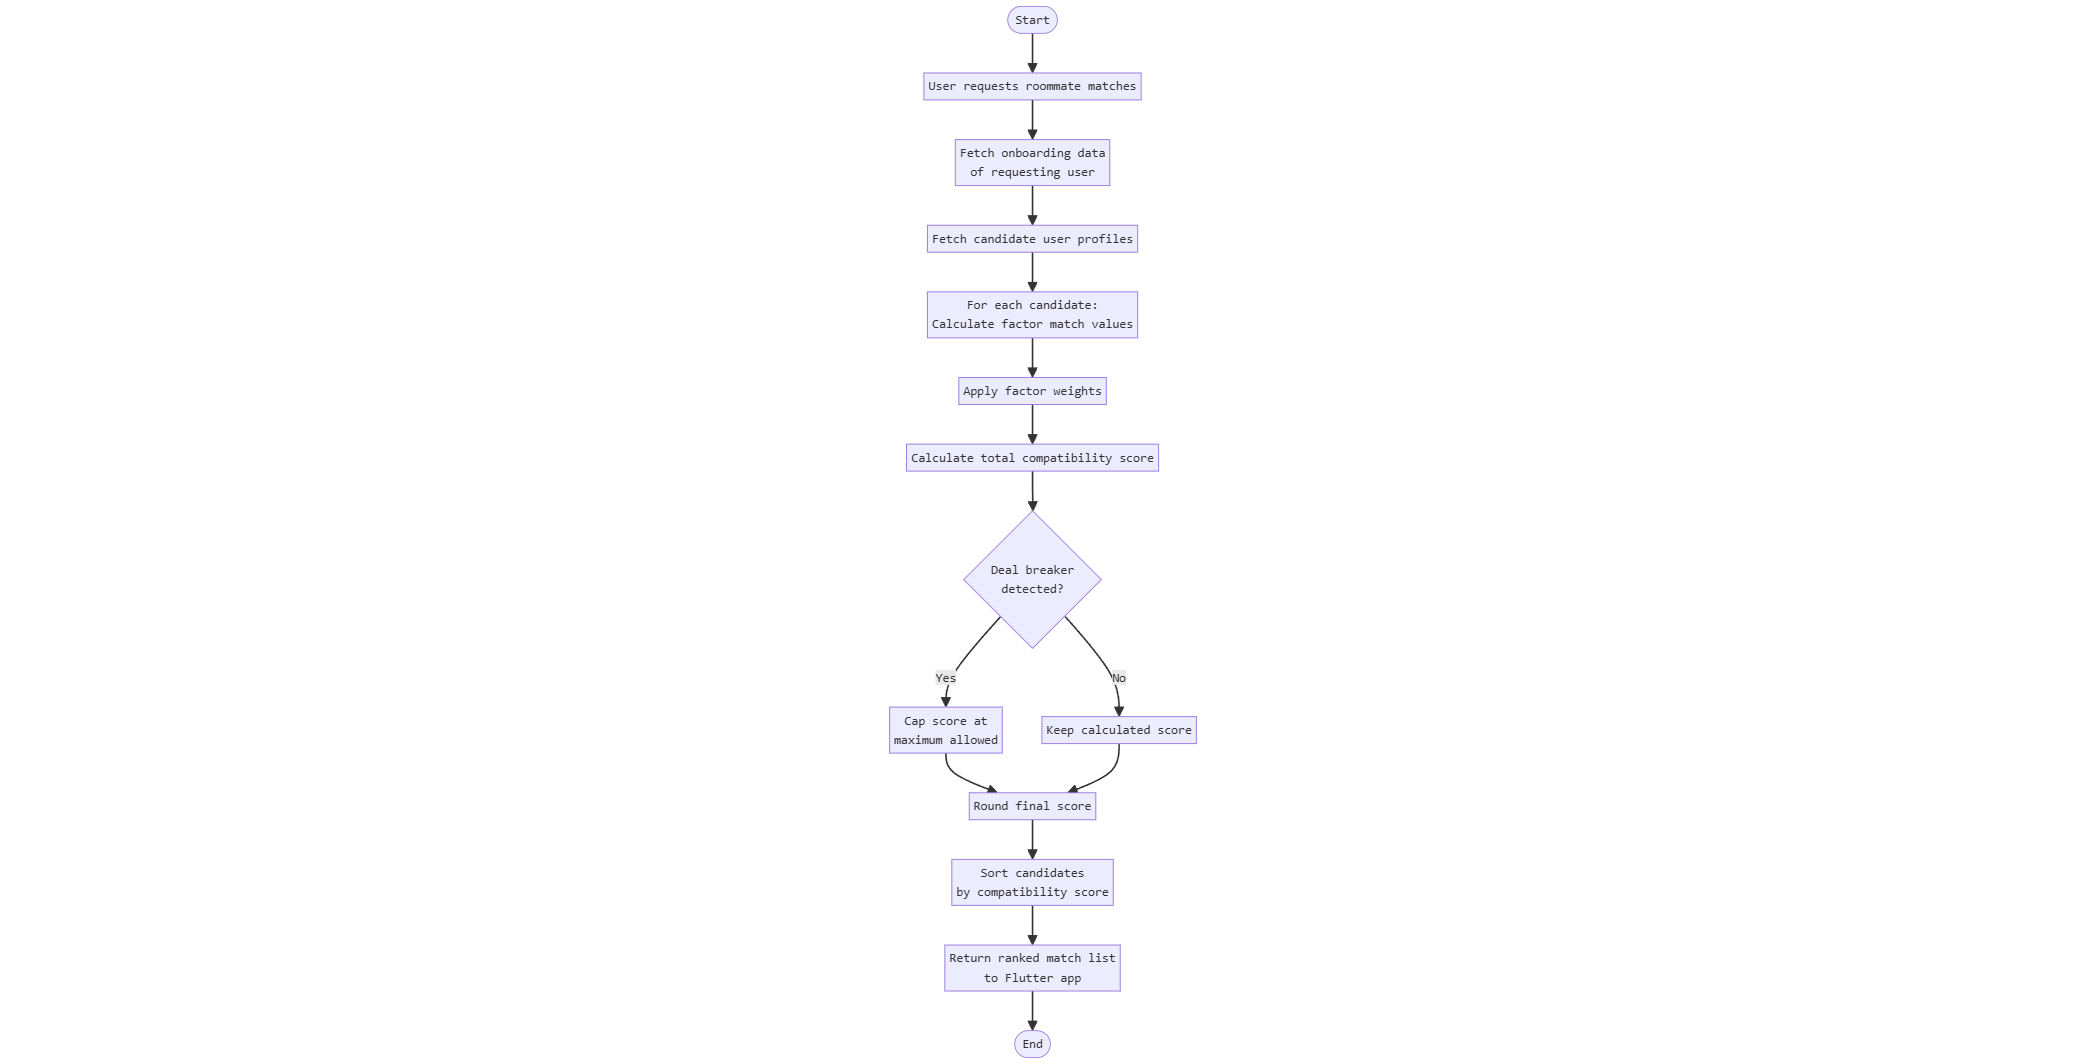
\includegraphics[width=1.0\textwidth, keepaspectratio]{images/flowchart.png}
    \caption{System Flowchart}
    \label{fig:flowchart}
\end{figure}
The flowchart illustrates the step-by-step operational flow of the TRIBAL system.


\section{UML Diagrams}
\begin{figure}[H]
    \centering
    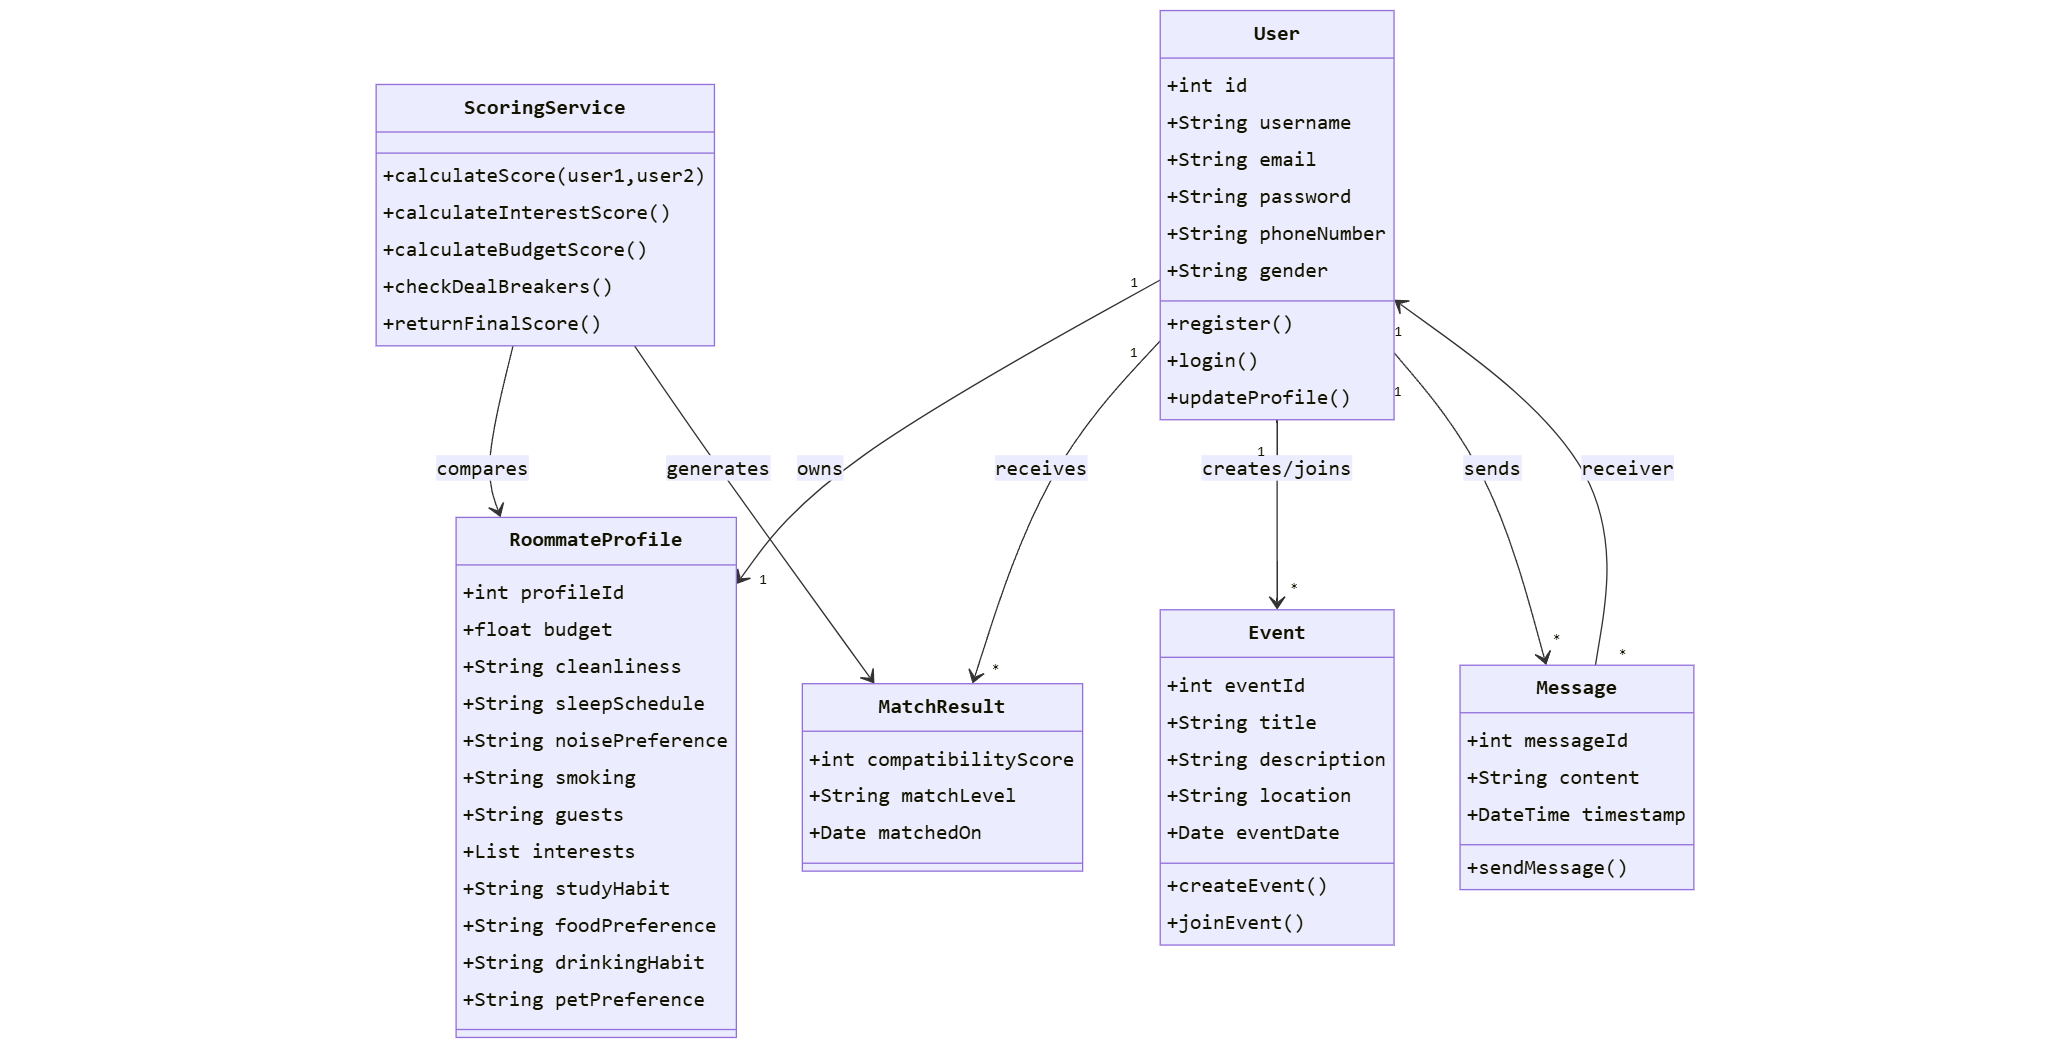
\includegraphics[width=0.95\textwidth]{images/uml.png}
    \caption{UML Diagram}
    \label{fig:uml_diagram}
\end{figure}
The UML diagram provides an object-oriented view of the system's architecture, showing key classes and their relationships.


\section{Tools Used}
The following tools and technologies are being used in the development of TRIBAL:
\begin{table}[H]
\centering
\begin{tabular}{|l|l|}
\hline
\textbf{Category} & \textbf{Tool / Technology} \\
\hline
Frontend Framework &  Flutter \\
Frontend Language &  Dart \\
State Management &  Provider \\
Navigation &  GoRouter \\
Backend Framework &  Django \\
Backend Language &  Python \\
Database &  PostgreSQL \\
Authentication &  JWT \\
Real-Time Communication &  Django Channels, WebSockets \\
Version Control &  Git, GitHub \\
Code Editor &  Visual Studio Code \\
Mobile Testing &  Android Studio \\
API Testing &  Postman \\
UI/UX Design &   Figma \\
\hline
\end{tabular}
\caption{Tools and Technologies Used}
\label{table:tools_used}
\end{table}
Flutter was chosen for the frontend because it allows the team to write one codebase that works on both Android and iOS. Django was chosen for the backend because it comes with many built-in features like an ORM and an admin panel, which makes development faster for a project with this scope. PostgreSQL was chosen as the database because it works well with Django and can reliably handle relational data like user profiles and onboarding responses.

 
 \chapter{Epilogue}

\section{Tasks Completed}
So far, the team has completed the following tasks:
\begin{itemize}
\item UI design for onboarding, login, signup, and profile setup screens in Flutter.
\item Implementation of the three-slide onboarding screen with skip and next functionality.
\item Animated loading screen shown during navigation between major flows.
\item Django project setup with PostgreSQL as the database.
\item JWT-based authentication APIs for login and signup.
\item Database models for User and RoommateProfile.
\item Design of the roommate compatibility scoring algorithm with weighted factors and deal breaker rules.

\item Manual API testing using Postman.
\item GitHub repository setup for version control and team collaboration.
\end{itemize}

\section{Remaining Tasks}
The following tasks are still remaining and will be completed in the upcoming sprints before the final defense:
\begin{itemize}
\item Implementation of the scoring logic inside the roommate module (models, scoring, services, views, serializers, urls, admin).
\item Initial unit tests for the scoring function.
\item Integration of the roommate matching API with the Flutter frontend, so that real compatibility scores are shown in the app instead of placeholder data.

\item Implementation of the real-time chat system using Django Channels and WebSockets.
\item Chat screens in Flutter for one-to-one conversations between matched users.
\item Event creation and joining module, including event listing and filtering screens.
\item Notification system for new matches and messages.

\item Full integration testing between the Flutter frontend and the Django backend.
\item Final round of bug fixing and performance testing.
\item Preparation of the user manual and final project documentation.
\item Deployment of the backend and preparation for the final presentation.
\end{itemize}

\section{Updated Gantt Chart}
The original time schedule has been adjusted slightly based on the actual pace of development so far. The updated schedule below shows the completed sprints and the plan for the remaining weeks leading up to the final defense.


\begin{center}
\resizebox{1.0\textwidth}{!}{%
\begin{tabular}{|p{0.30\textwidth}*{7}{|p{0.035\textwidth}}|!{\color{red}\vrule width 1.5pt height 5pt depth 1pt}p{0.035\textwidth}*{4}{|p{0.035\textwidth}}|}
 \hline
 \textbf{Tasks} & \multicolumn{12}{c|}{\textbf{Weeks}} \\
 \hline
 & 2 & 4 & 6 & 8 & 10 & 12 & 14 & 16 & 18 & 20 & 22 & 24 \\
 \hline
Requirement Analysis \on{2}\off{10} \\
 \hline
System Design \off{2}\on{2}\off{8} \\
 \hline
Implementation \off{4}\on{4}\off{4} \\
 \hline
Testing and Evaluation \off{7}\on{3}\off{2} \\
 \hline
Deployment \off{10}\on{1}\off{1} \\
 \hline
Monitoring\off{11}\on{1} \\
 \hline
Documentation \on{12} \\
\hline
\end{tabular}}
\end{center}

The team is currently on Sprint 5. Based on the progress made so far, the team is confident that the remaining sprints can be completed within the original 16-week timeline, with some buffer time set aside before the final defense for bug fixing and documentation.

 
\backmatter
\emergencystretch=1em

\nocite{*}
\printbibliography[heading=bibintoc, title={References and Bibliography}]

\newpage

\chapter*{Screenshots}
\addcontentsline{toc}{chapter}{Screenshots}

\begin{figure}[H]
    \centering
    \begin{subfigure}{0.35\textwidth}
        \centering
        
\includegraphics[width=0.8\textwidth]{images/ss/ss1.png}
        \caption{Screenshot 1}
        \label{fig:ss1}
    \end{subfigure}
    \hfill
    \begin{subfigure}{0.35\textwidth}
        \centering
        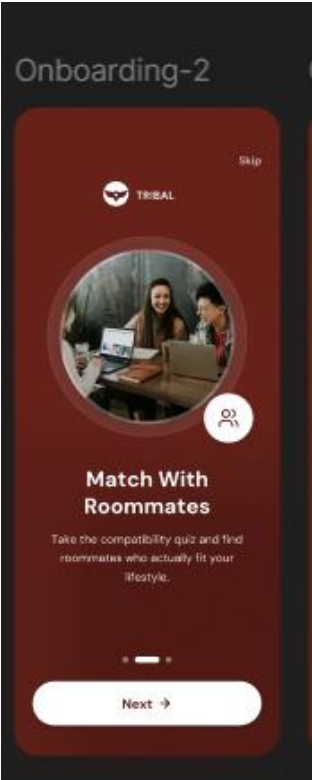
\includegraphics[width=0.8\textwidth]{images/ss/ss2.png}
        \caption{Screenshot 2}
        \label{fig:ss2}
    \end{subfigure}
    \caption{TRIBAL Application Screenshots (Part 1)}
    \label{fig:all_screenshots1}
\end{figure}

\begin{figure}[H]
    \centering
    \begin{subfigure}{0.35\textwidth}
        \centering
        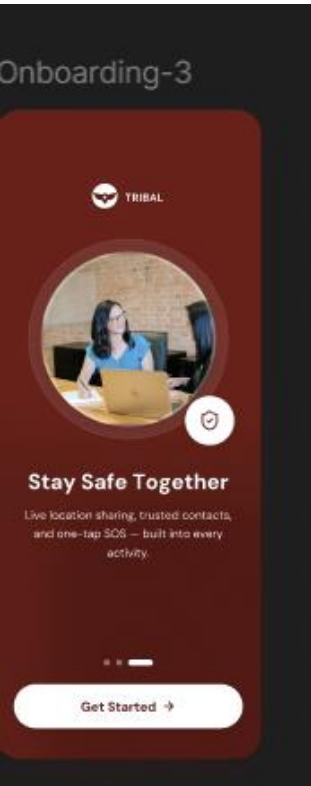
\includegraphics[width=0.8\textwidth]{images/ss/ss3.png}
        \caption{Screenshot 3}
        \label{fig:ss3}
    \end{subfigure}
    \hfill
    \begin{subfigure}{0.35\textwidth}
        \centering
        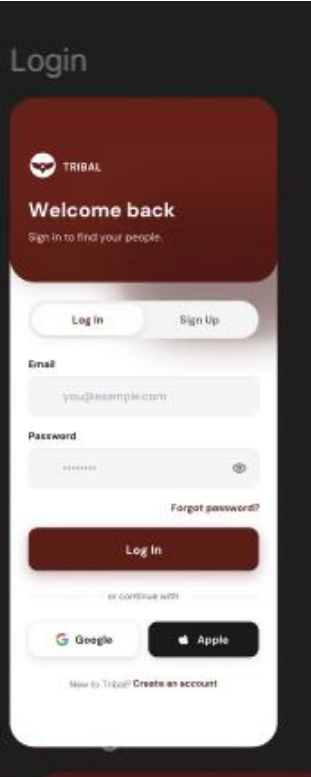
\includegraphics[width=0.8\textwidth]{images/ss/ss4.png}
        \caption{Screenshot 4}
        \label{fig:ss4}
    \end{subfigure}
    \caption{TRIBAL Application Screenshots (Part 2)}
    \label{fig:all_screenshots2}
\end{figure}

\begin{figure}[H]
    \centering
    \begin{subfigure}{0.35\textwidth}
        \centering
        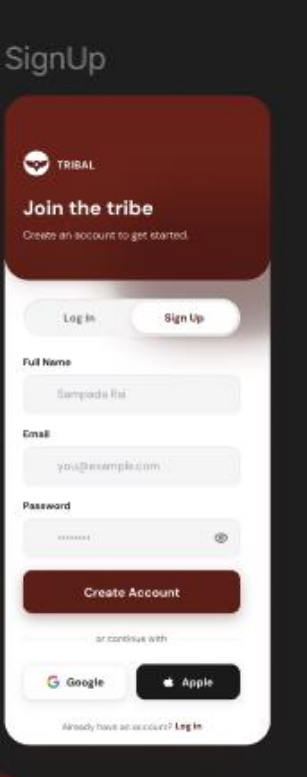
\includegraphics[width=0.8\textwidth]{images/ss/ss5.png}
        \caption{Screenshot 5}
        \label{fig:ss5}
    \end{subfigure}
    \hfill
    \begin{subfigure}{0.35\textwidth}
        \centering
        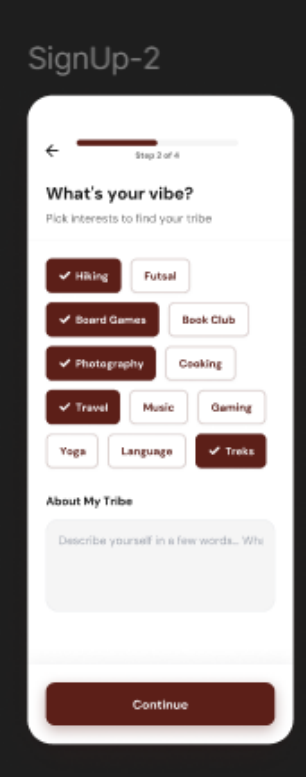
\includegraphics[width=0.8\textwidth]{images/ss/ss6.png}
        \caption{Screenshot 6}
        \label{fig:ss6}
    \end{subfigure}
    \caption{TRIBAL Application Screenshots (Part 3)}
    \label{fig:all_screenshots3}
\end{figure}


\end{document}
